\documentclass[border=10pt,tikz]{standalone}
\usepackage[T1]{fontenc}
\usepackage{tikz}
\usetikzlibrary{
  positioning, arrows.meta, calc, fit, backgrounds,
  shapes.geometric, shapes.multipart, decorations.pathmorphing,
  decorations.markings, patterns, shadows.blur
}
\usepackage{xcolor}
\usepackage{amsmath,amssymb}

% ── Colour palette ──────────────────────────────────────────
\definecolor{userBg}{HTML}{E3F2FD}
\definecolor{userBdr}{HTML}{1565C0}
\definecolor{entBg}{HTML}{FFF3E0}
\definecolor{entBdr}{HTML}{E65100}
\definecolor{opBg}{HTML}{FCE4EC}
\definecolor{opBdr}{HTML}{B71C1C}
\definecolor{dmzBg}{HTML}{E8F5E9}
\definecolor{dmzBdr}{HTML}{2E7D32}
\definecolor{resBg}{HTML}{F3E5F5}
\definecolor{resBdr}{HTML}{6A1B9A}

\definecolor{redAgent}{HTML}{D32F2F}
\definecolor{blueAgent}{HTML}{1565C0}
\definecolor{greenAgent}{HTML}{2E7D32}
\definecolor{fwRed}{HTML}{C62828}
\definecolor{dqnBg}{HTML}{E8EAF6}
\definecolor{dqnBdr}{HTML}{283593}

\definecolor{winColor}{HTML}{1565C0}
\definecolor{lnxColor}{HTML}{388E3C}
\definecolor{gwColor}{HTML}{00695C}
\definecolor{srvColor}{HTML}{E65100}
\definecolor{monColor}{HTML}{6A1B9A}

% ── TikZ styles ─────────────────────────────────────────────
\tikzset{
  host/.style={
    draw=gray!70, rounded corners=2pt, minimum width=1.8cm,
    minimum height=0.7cm, font=\scriptsize\bfseries, inner sep=2pt,
    blur shadow={shadow blur steps=3, shadow xshift=0.5pt,
                 shadow yshift=-0.5pt, shadow blur radius=1pt}
  },
  winhost/.style={host, fill=userBg!50},
  lnxhost/.style={host, fill=dmzBg!50},
  srvhost/.style={host, fill=entBg!40},
  gwhost/.style={host, fill=yellow!8},
  monhost/.style={host, fill=opBg!30},
  subnet/.style 2 args={
    draw=#2, line width=1.2pt, rounded corners=6pt,
    fill=#1, inner sep=10pt
  },
  subnetlabel/.style={
    font=\small\bfseries, fill=white, fill opacity=0.92,
    text opacity=1, rounded corners=2pt, inner sep=3pt
  },
  agentbox/.style 2 args={
    draw=#1, line width=1.5pt, rounded corners=6pt,
    fill=white, inner sep=8pt, text width=#2
  },
  agenttitle/.style={
    font=\normalsize\bfseries, text=white, fill=#1,
    rounded corners=3pt, inner sep=4pt, anchor=north
  },
  fwlabel/.style={
    font=\tiny\bfseries, text=fwRed, fill=red!5,
    draw=fwRed, rounded corners=1.5pt, inner sep=2pt, align=center
  },
  attackarrow/.style={
    -{Stealth[length=5pt]}, redAgent, line width=1.2pt, dashed
  },
  defendarrow/.style={
    -{Stealth[length=4pt]}, blueAgent, line width=1pt, opacity=0.7
  },
  netarrow/.style={
    {Stealth[length=4pt]}-{Stealth[length=4pt]}, gray!60, line width=1.2pt
  },
  ostag/.style={font=\fontsize{4.5}{5}\selectfont\bfseries},
}

\begin{document}
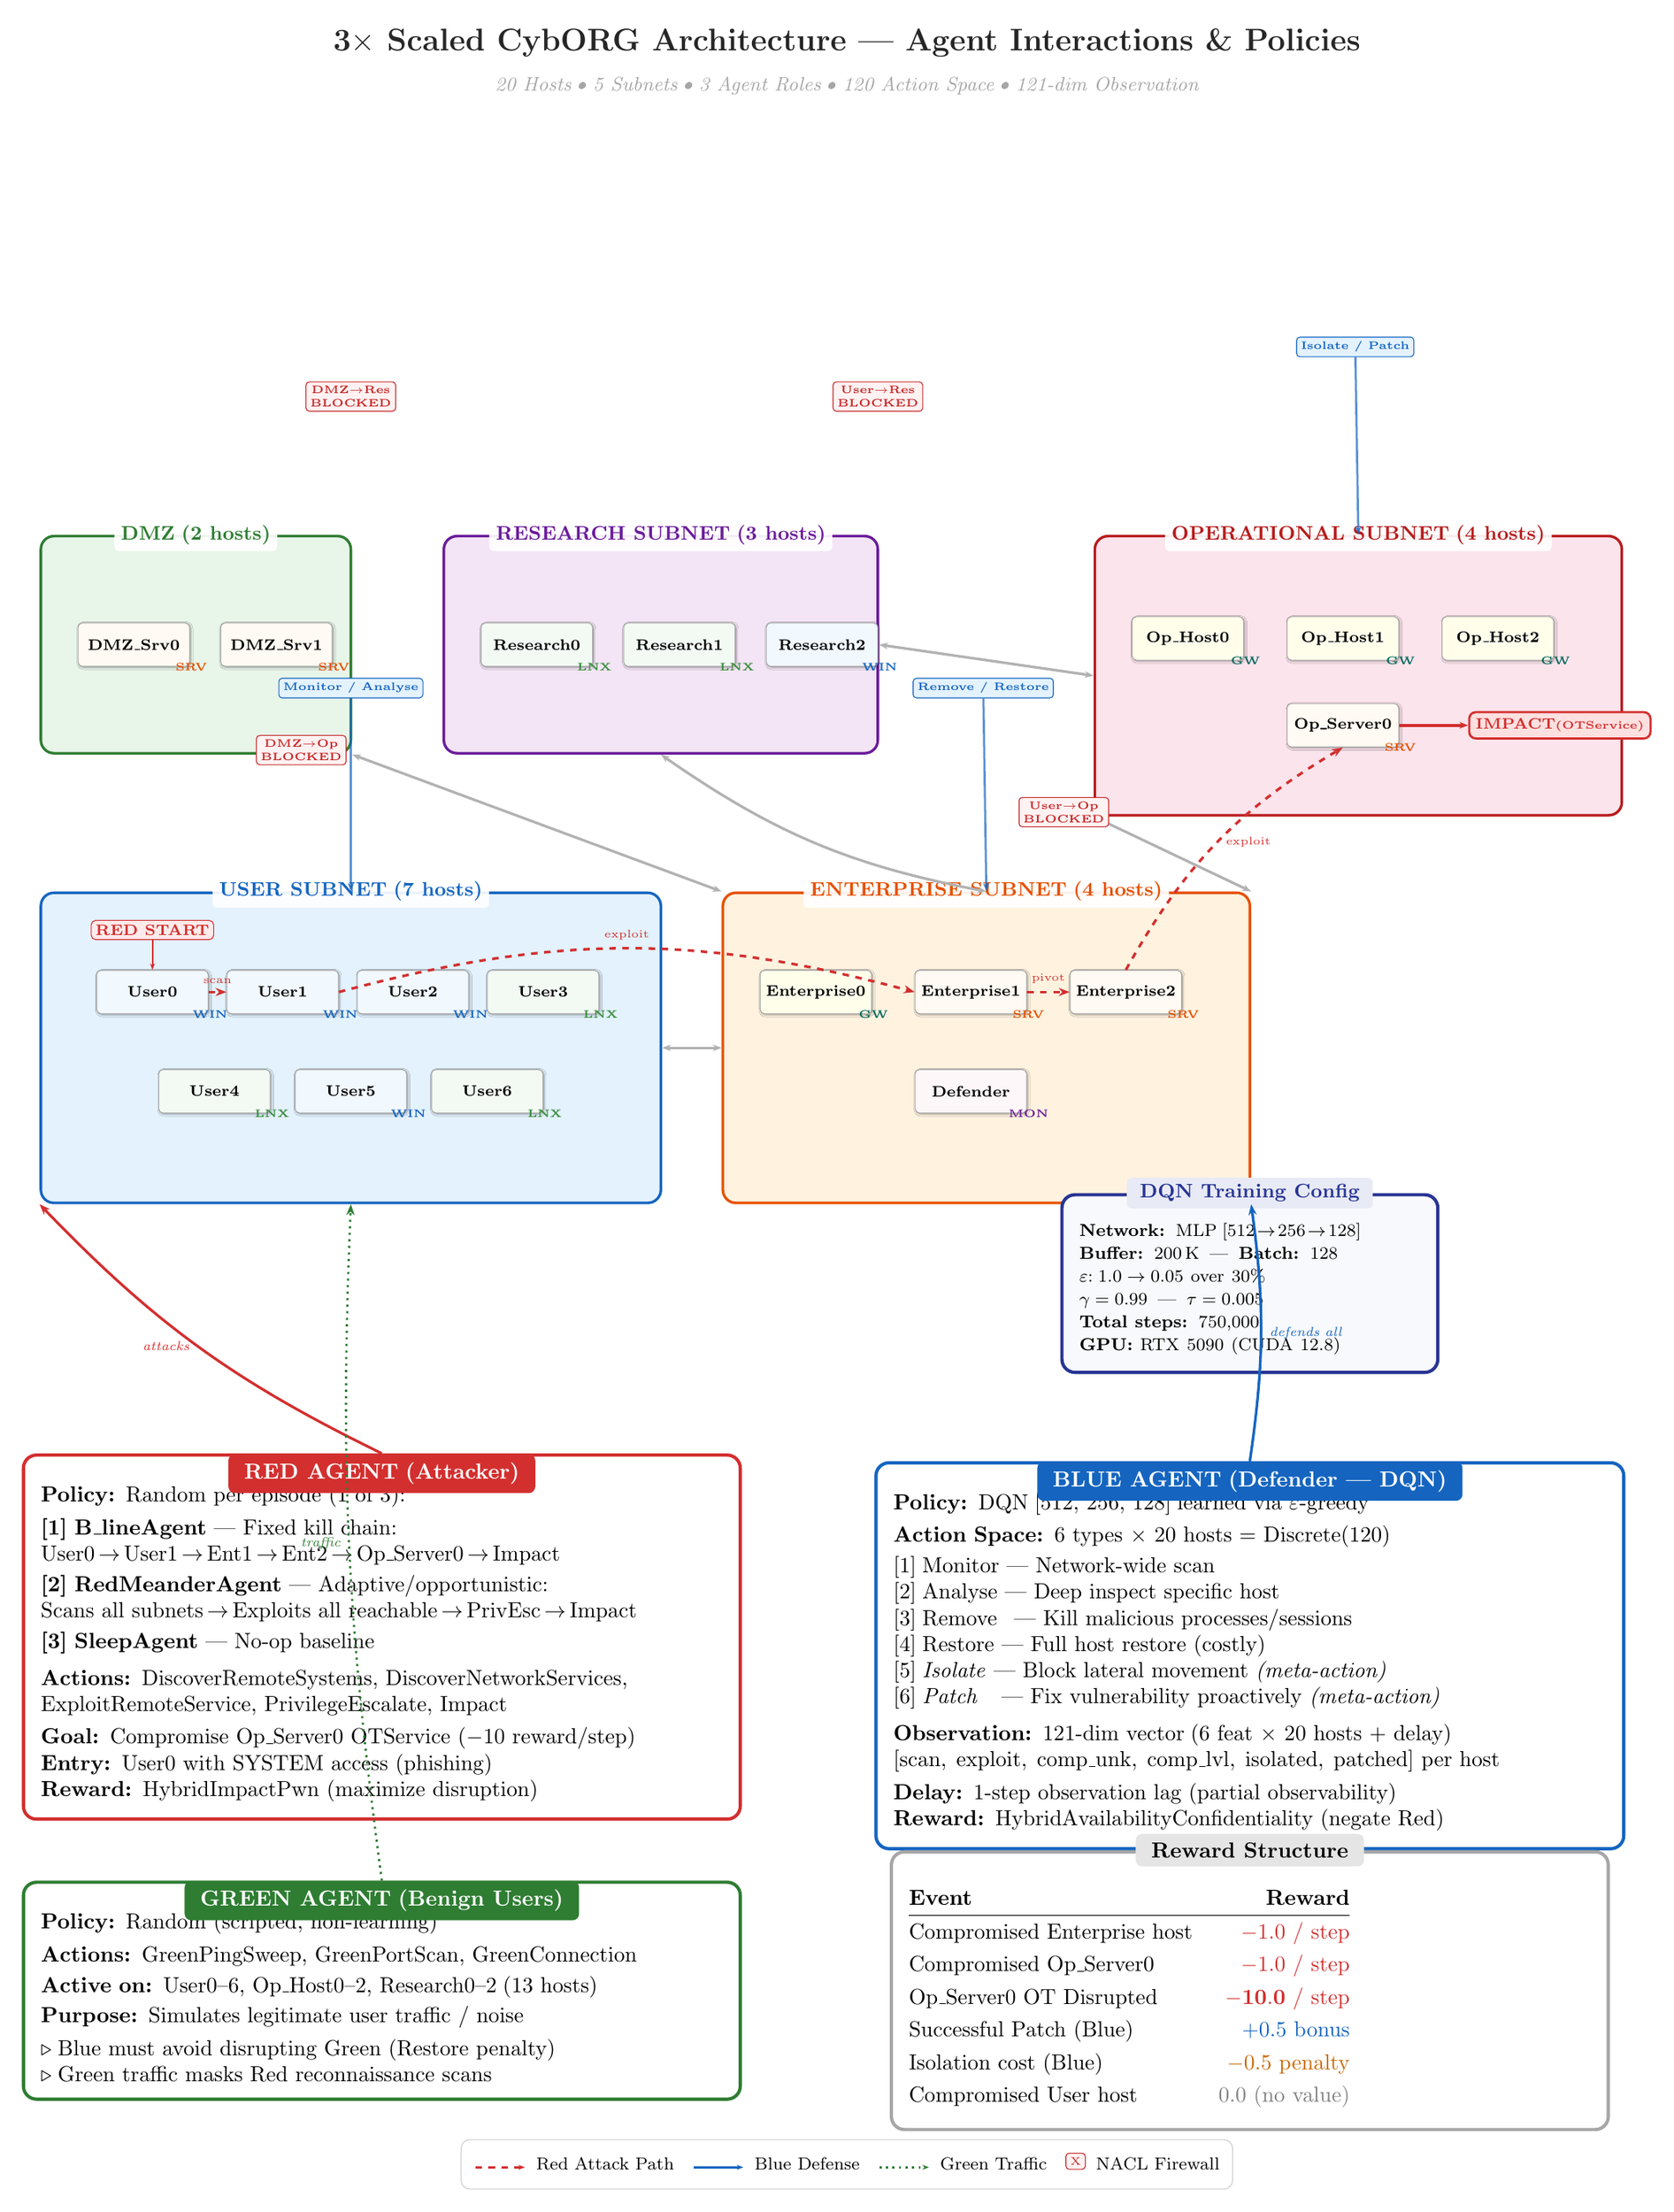
\begin{tikzpicture}[x=1cm, y=1cm]

% ════════════════════════════════════════════════════════════
%  TITLE
% ════════════════════════════════════════════════════════════
\node[font=\Large\bfseries, text=black!85] at (13,22.2)
  {3$\times$ Scaled CybORG Architecture --- Agent Interactions \& Policies};
\node[font=\small\itshape, text=gray!70] at (13,21.5)
  {20 Hosts\;\textbullet\;5 Subnets\;\textbullet\;3 Agent Roles%
   \;\textbullet\;120 Action Space\;\textbullet\;121-dim Observation};

% ════════════════════════════════════════════════════════════
%  USER SUBNET  (7 hosts)
% ════════════════════════════════════════════════════════════
\begin{scope}[shift={(0,6)}]
  \node[subnet={userBg}{userBdr}, minimum width=10cm,
        minimum height=5cm] (usub) at (5,0) {};
  \node[subnetlabel, text=userBdr] at (usub.north) {USER SUBNET\;(7 hosts)};

  \node[winhost] (U0) at (1.8, 0.9)  {User0};
  \node[winhost] (U1) at (3.9, 0.9)  {User1};
  \node[winhost] (U2) at (6.0, 0.9)  {User2};
  \node[lnxhost] (U3) at (8.1, 0.9)  {User3};
  \node[lnxhost] (U4) at (2.8,-0.7)  {User4};
  \node[winhost] (U5) at (5.0,-0.7)  {User5};
  \node[lnxhost] (U6) at (7.2,-0.7)  {User6};

  % OS tags
  \node[ostag, text=winColor] at (U0.south east) {\,WIN};
  \node[ostag, text=winColor] at (U1.south east) {\,WIN};
  \node[ostag, text=winColor] at (U2.south east) {\,WIN};
  \node[ostag, text=lnxColor] at (U3.south east) {\,LNX};
  \node[ostag, text=lnxColor] at (U4.south east) {\,LNX};
  \node[ostag, text=winColor] at (U5.south east) {\,WIN};
  \node[ostag, text=lnxColor] at (U6.south east) {\,LNX};

  % Red START marker
  \node[font=\scriptsize\bfseries, text=redAgent, fill=red!8,
        draw=redAgent, rounded corners=2pt, inner sep=2pt]
    (redstart) at (1.8, 1.9) {RED START};
  \draw[-{Stealth[length=3pt]}, redAgent, thick] (redstart) -- (U0);
\end{scope}

% ════════════════════════════════════════════════════════════
%  ENTERPRISE SUBNET  (4 hosts)
% ════════════════════════════════════════════════════════════
\begin{scope}[shift={(11,6)}]
  \node[subnet={entBg}{entBdr}, minimum width=8.5cm,
        minimum height=5cm] (esub) at (4.25,0) {};
  \node[subnetlabel, text=entBdr] at (esub.north)
    {ENTERPRISE SUBNET\;(4 hosts)};

  \node[gwhost]  (E0) at (1.5, 0.9)  {Enterprise0};
  \node[srvhost] (E1) at (4.0, 0.9)  {Enterprise1};
  \node[srvhost] (E2) at (6.5, 0.9)  {Enterprise2};
  \node[monhost] (Def) at (4.0,-0.7) {Defender};

  \node[ostag, text=gwColor]  at (E0.south east)  {\,GW};
  \node[ostag, text=srvColor] at (E1.south east)  {\,SRV};
  \node[ostag, text=srvColor] at (E2.south east)  {\,SRV};
  \node[ostag, text=monColor] at (Def.south east)  {\,MON};
\end{scope}

% ════════════════════════════════════════════════════════════
%  OPERATIONAL SUBNET  (4 hosts)
% ════════════════════════════════════════════════════════════
\begin{scope}[shift={(17,12)}]
  \node[subnet={opBg}{opBdr}, minimum width=8.5cm,
        minimum height=4.5cm] (osub) at (4.25,0) {};
  \node[subnetlabel, text=opBdr] at (osub.north)
    {OPERATIONAL SUBNET\;(4 hosts)};

  \node[gwhost]  (OH0) at (1.5, 0.6)  {Op\_Host0};
  \node[gwhost]  (OH1) at (4.0, 0.6)  {Op\_Host1};
  \node[gwhost]  (OH2) at (6.5, 0.6)  {Op\_Host2};
  \node[srvhost] (OS0) at (4.0,-0.8)  {Op\_Server0};

  \node[ostag, text=gwColor]  at (OH0.south east) {\,GW};
  \node[ostag, text=gwColor]  at (OH1.south east) {\,GW};
  \node[ostag, text=gwColor]  at (OH2.south east) {\,GW};
  \node[ostag, text=srvColor] at (OS0.south east) {\,SRV};

  % IMPACT marker
  \node[font=\scriptsize\bfseries, text=redAgent, fill=red!12,
        draw=redAgent, rounded corners=3pt, inner sep=3pt,
        line width=1pt]
    (impact) at (7.5,-0.8) {\textbf{IMPACT}\\[-1pt]{\fontsize{5}{6}\selectfont(OTService)}};
  \draw[-{Stealth[length=4pt]}, redAgent, line width=1.5pt] (OS0) -- (impact);
\end{scope}

% ════════════════════════════════════════════════════════════
%  DMZ SUBNET  (2 hosts)
% ════════════════════════════════════════════════════════════
\begin{scope}[shift={(0,12.5)}]
  \node[subnet={dmzBg}{dmzBdr}, minimum width=5cm,
        minimum height=3.5cm] (dsub) at (2.5,0) {};
  \node[subnetlabel, text=dmzBdr] at (dsub.north) {DMZ\;(2 hosts)};

  \node[srvhost] (DZ0) at (1.5, 0.0) {DMZ\_Srv0};
  \node[srvhost] (DZ1) at (3.8, 0.0) {DMZ\_Srv1};

  \node[ostag, text=srvColor] at (DZ0.south east) {\,SRV};
  \node[ostag, text=srvColor] at (DZ1.south east) {\,SRV};
\end{scope}

% ════════════════════════════════════════════════════════════
%  RESEARCH SUBNET  (3 hosts)
% ════════════════════════════════════════════════════════════
\begin{scope}[shift={(6.5,12.5)}]
  \node[subnet={resBg}{resBdr}, minimum width=7cm,
        minimum height=3.5cm] (rsub) at (3.5,0) {};
  \node[subnetlabel, text=resBdr] at (rsub.north)
    {RESEARCH SUBNET\;(3 hosts)};

  \node[lnxhost] (R0) at (1.5, 0.0) {Research0};
  \node[lnxhost] (R1) at (3.8, 0.0) {Research1};
  \node[winhost] (R2) at (6.1, 0.0) {Research2};

  \node[ostag, text=lnxColor] at (R0.south east) {\,LNX};
  \node[ostag, text=lnxColor] at (R1.south east) {\,LNX};
  \node[ostag, text=winColor] at (R2.south east) {\,WIN};
\end{scope}

% ════════════════════════════════════════════════════════════
%  INTER-SUBNET CONNECTIONS
% ════════════════════════════════════════════════════════════
% User <-> Enterprise
\draw[netarrow] (usub.east) -- (esub.west);
% Enterprise <-> Operational
\draw[netarrow] (esub.north east) -- (osub.south west);
% Enterprise <-> DMZ
\draw[netarrow] (esub.north west) -- (dsub.south east);
% Enterprise <-> Research
\draw[netarrow] (esub.north) to[bend left=12] (rsub.south);
% Research <-> Operational
\draw[netarrow] (rsub.east) -- (osub.west);

% ════════════════════════════════════════════════════════════
%  NACL FIREWALLS
% ════════════════════════════════════════════════════════════
\node[fwlabel] at (16.5, 9.8) {User$\to$Op\\BLOCKED};
\node[fwlabel] at (4.2, 10.8) {DMZ$\to$Op\\BLOCKED};
\node[fwlabel] at (13.5, 16.5) {User$\to$Res\\BLOCKED};
\node[fwlabel] at (5.0, 16.5) {DMZ$\to$Res\\BLOCKED};

% ════════════════════════════════════════════════════════════
%  RED ATTACK PATH  (B_line kill chain)
% ════════════════════════════════════════════════════════════
\draw[attackarrow] (U0.east) -- node[above, font=\fontsize{5}{6}\selectfont,
  text=redAgent] {scan} (U1.west);
\draw[attackarrow] (U1.east) to[bend left=15]
  node[above, font=\fontsize{5}{6}\selectfont, text=redAgent] {exploit}
  (E1.west);
\draw[attackarrow] (E1.east) --
  node[above, font=\fontsize{5}{6}\selectfont, text=redAgent] {pivot}
  (E2.west);
\draw[attackarrow] (E2.north) to[bend left=15]
  node[right, font=\fontsize{5}{6}\selectfont, text=redAgent] {exploit}
  (OS0.south);

% ════════════════════════════════════════════════════════════
%  BLUE DEFENSE ARROWS
% ════════════════════════════════════════════════════════════
\node[font=\fontsize{5.5}{6.5}\selectfont\bfseries, text=blueAgent,
      fill=userBg, draw=blueAgent, rounded corners=1.5pt, inner sep=2pt]
  (bm1) at (5, 11.8) {Monitor / Analyse};
\draw[defendarrow] (bm1) -- (usub.north);

\node[font=\fontsize{5.5}{6.5}\selectfont\bfseries, text=blueAgent,
      fill=userBg, draw=blueAgent, rounded corners=1.5pt, inner sep=2pt]
  (bm2) at (15.2, 11.8) {Remove / Restore};
\draw[defendarrow] (bm2) -- (esub.north);

\node[font=\fontsize{5.5}{6.5}\selectfont\bfseries, text=blueAgent,
      fill=userBg, draw=blueAgent, rounded corners=1.5pt, inner sep=2pt]
  (bm3) at (21.2, 17.3) {Isolate / Patch};
\draw[defendarrow] (bm3) -- (osub.north);

% ════════════════════════════════════════════════════════════
%  RED AGENT INFO BOX
% ════════════════════════════════════════════════════════════
\node[agentbox={redAgent}{11cm}] (redbox) at (5.5, -3.5) {
  \begin{minipage}{10.8cm}
  \vspace{6pt}
  \textbf{Policy:} Random per episode (1 of 3):\\[3pt]
  \quad\textbf{[1] B\_lineAgent} --- Fixed kill chain:\\
  \quad\quad User0\,$\to$\,User1\,$\to$\,Ent1\,$\to$\,Ent2\,%
  $\to$\,Op\_Server0\,$\to$\,Impact\\[2pt]
  \quad\textbf{[2] RedMeanderAgent} --- Adaptive/opportunistic:\\
  \quad\quad Scans all subnets\,$\to$\,Exploits all reachable\,%
  $\to$\,PrivEsc\,$\to$\,Impact\\[2pt]
  \quad\textbf{[3] SleepAgent} --- No-op baseline\\[5pt]
  \textbf{Actions:} DiscoverRemoteSystems, DiscoverNetworkServices,\\
  \quad ExploitRemoteService, PrivilegeEscalate, Impact\\[3pt]
  \textbf{Goal:} Compromise Op\_Server0 OTService ($-10$ reward/step)\\
  \textbf{Entry:} User0 with SYSTEM access (phishing)\\
  \textbf{Reward:} HybridImpactPwn (maximize disruption)
  \end{minipage}
};
\node[agenttitle=redAgent] at (redbox.north) {\;RED AGENT\;(Attacker)\;};

% ════════════════════════════════════════════════════════════
%  BLUE AGENT INFO BOX
% ════════════════════════════════════════════════════════════
\node[agentbox={blueAgent}{11.5cm}] (bluebox) at (19.5, -3.8) {
  \begin{minipage}{11.2cm}
  \vspace{6pt}
  \textbf{Policy:} DQN\;$[512,\,256,\,128]$\;learned via
    $\varepsilon$-greedy\\[3pt]
  \textbf{Action Space:} $6$ types $\times$ $20$ hosts
    $=$ Discrete($120$)\\[2pt]
  \quad [1]\;Monitor --- Network-wide scan\\
  \quad [2]\;Analyse --- Deep inspect specific host\\
  \quad [3]\;Remove\;\, --- Kill malicious processes/sessions\\
  \quad [4]\;Restore --- Full host restore (costly)\\
  \quad [5]\;\textit{Isolate} --- Block lateral movement
    \textit{(meta-action)}\\
  \quad [6]\;\textit{Patch}\;\;\, --- Fix vulnerability proactively
    \textit{(meta-action)}\\[5pt]
  \textbf{Observation:} 121-dim vector\;%
    ($6$ feat $\times$ $20$ hosts $+$ delay)\\
  \quad$[\text{scan},\;\text{exploit},\;\text{comp\_unk},\;%
    \text{comp\_lvl},\;\text{isolated},\;\text{patched}]$
    per host\\[3pt]
  \textbf{Delay:} 1-step observation lag (partial observability)\\
  \textbf{Reward:} HybridAvailabilityConfidentiality (negate Red)
  \end{minipage}
};
\node[agenttitle=blueAgent] at (bluebox.north)
  {\;BLUE AGENT\;(Defender --- DQN)\;};

% ════════════════════════════════════════════════════════════
%  GREEN AGENT INFO BOX
% ════════════════════════════════════════════════════════════
\node[agentbox={greenAgent}{11cm}] (greenbox) at (5.5, -9.2) {
  \begin{minipage}{10.8cm}
  \vspace{6pt}
  \textbf{Policy:} Random (scripted, non-learning)\\[3pt]
  \textbf{Actions:} GreenPingSweep, GreenPortScan, GreenConnection\\[2pt]
  \textbf{Active on:} User0--6, Op\_Host0--2, Research0--2\;(13 hosts)\\[2pt]
  \textbf{Purpose:} Simulates legitimate user traffic / noise\\[3pt]
  $\triangleright$\;Blue must avoid disrupting Green
    (Restore penalty)\\
  $\triangleright$\;Green traffic masks Red reconnaissance scans
  \end{minipage}
};
\node[agenttitle=greenAgent] at (greenbox.north)
  {\;GREEN AGENT\;(Benign Users)\;};

% ════════════════════════════════════════════════════════════
%  REWARD STRUCTURE BOX
% ════════════════════════════════════════════════════════════
\node[agentbox={gray!70}{11cm}] (rewbox) at (19.5, -9.2) {
  \begin{minipage}{10.8cm}
  \vspace{6pt}
  \renewcommand{\arraystretch}{1.25}
  \begin{tabular}{@{}l r@{}}
  \textbf{Event} & \textbf{Reward}\\
  \hline
  Compromised Enterprise host & \textcolor{redAgent}{$-1.0$ / step}\\
  Compromised Op\_Server0      & \textcolor{redAgent}{$-1.0$ / step}\\
  Op\_Server0 OT Disrupted     & \textcolor{redAgent}{$\mathbf{-10.0}$ / step}\\
  Successful Patch (Blue)      & \textcolor{blueAgent}{$+0.5$ bonus}\\
  Isolation cost (Blue)        & \textcolor{orange!80!black}{$-0.5$ penalty}\\
  Compromised User host        & \textcolor{gray}{$0.0$ (no value)}\\
  \end{tabular}
  \end{minipage}
};
\node[font=\normalsize\bfseries, fill=gray!20, rounded corners=3pt,
      inner sep=4pt] at (rewbox.north) {\;Reward Structure\;};

% ════════════════════════════════════════════════════════════
%  DQN TRAINING CONFIG BOX
% ════════════════════════════════════════════════════════════
\node[agentbox={dqnBdr}{5.5cm}, fill=dqnBg!30] (dqnbox) at (19.5, 2.2) {
  \begin{minipage}{5.2cm}
  \vspace{5pt}
  \footnotesize
  \textbf{Network:} MLP\;$[512\!\to\!256\!\to\!128]$\\[1pt]
  \textbf{Buffer:} 200\,K\;\;|\;\;\textbf{Batch:} 128\\[1pt]
  $\varepsilon$:\;$1.0 \to 0.05$ over 30\%\\[1pt]
  $\gamma = 0.99$\;\;|\;\;$\tau = 0.005$\\[1pt]
  \textbf{Total steps:} 750{,}000\\[1pt]
  \textbf{GPU:} RTX 5090 (CUDA 12.8)
  \end{minipage}
};
\node[font=\small\bfseries, text=dqnBdr, fill=dqnBg,
      rounded corners=2pt, inner sep=3pt] at (dqnbox.north)
  {\;DQN Training Config\;};

% ════════════════════════════════════════════════════════════
%  INTERACTION ARROWS  (Agent <-> Network)
% ════════════════════════════════════════════════════════════
% Red -> User subnet
\draw[-{Stealth[length=5pt]}, redAgent, line width=1.2pt]
  (redbox.north) to[bend left=10]
  node[midway, left, font=\fontsize{6}{7}\selectfont\itshape, text=redAgent]
  {attacks} (usub.south west);

% Blue -> All subnets (from blue box upward)
\draw[-{Stealth[length=5pt]}, blueAgent, line width=1.2pt]
  (bluebox.north) to[bend right=8]
  node[midway, right, font=\fontsize{6}{7}\selectfont\itshape, text=blueAgent]
  {defends all} (esub.south east);

% Green -> User/Op/Research
\draw[-{Stealth[length=5pt]}, greenAgent, line width=1pt, dotted]
  (greenbox.north) to[bend left=5]
  node[midway, left, font=\fontsize{6}{7}\selectfont\itshape, text=greenAgent]
  {traffic} (usub.south);

% ════════════════════════════════════════════════════════════
%  LEGEND
% ════════════════════════════════════════════════════════════
\node[draw=gray!40, rounded corners=4pt, fill=white, inner sep=6pt,
      font=\footnotesize] at (13, -12) {
  \begin{tabular}{@{}c@{\;\;}c@{\quad}c@{\;\;}c@{\quad}c@{\;\;}c@{\quad}c@{\;\;}c@{}}
    \tikz\draw[redAgent,dashed,line width=1pt,
      -{Stealth[length=3pt]}] (0,0)--(0.8,0); &
    Red Attack Path &
    \tikz\draw[blueAgent,line width=1pt,
      -{Stealth[length=3pt]}] (0,0)--(0.8,0); &
    Blue Defense &
    \tikz\draw[greenAgent,dotted,line width=1pt,
      -{Stealth[length=3pt]}] (0,0)--(0.8,0); &
    Green Traffic &
    \tikz\node[fwlabel,font=\fontsize{5}{6}\selectfont]{X}; &
    NACL Firewall
  \end{tabular}
};

\end{tikzpicture}
\end{document}
